% --- Distillation training: soft targets, temperature, and loss ---
\begin{frame}{Distillation: Soft Targets}
  \textbf{\textcolor{blue}{While training, our confidence in the labels must be high.}}\\[0.8em]
  Otherwise the data would not be present in the training set.\\[1em]
  \begin{columns}[T,onlytextwidth]
    \column{0.49\textwidth}
      \small
      For example: \\[0.7em]
      \texttt{This is a Dog}
      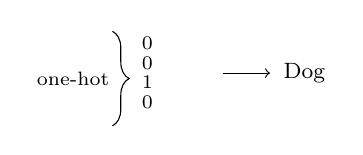
\begin{tikzpicture}[baseline={(0,0)}]
        % Draw brace + label for one-hot
        \draw[decorate,decoration={brace,amplitude=6pt,mirror}] (0,-0.2) -- (0,1) node[midway,xshift=-0.5cm] {\scriptsize one-hot};
        % One-hot vector
        \node[anchor=west] at (0.25,0.85) {\scriptsize 0};
        \node[anchor=west] at (0.25,0.60) {\scriptsize 0};
        \node[anchor=west] at (0.25,0.35) {\scriptsize 1};
        \node[anchor=west] at (0.25,0.10) {\scriptsize 0};
        % Arrow to "Dog"
        \draw[->] (1.4,0.47) -- (2,0.47);
        \node[anchor=west] at (2.05,0.47) {\footnotesize Dog};
      \end{tikzpicture}
    \column{0.48\textwidth}
      \centering
      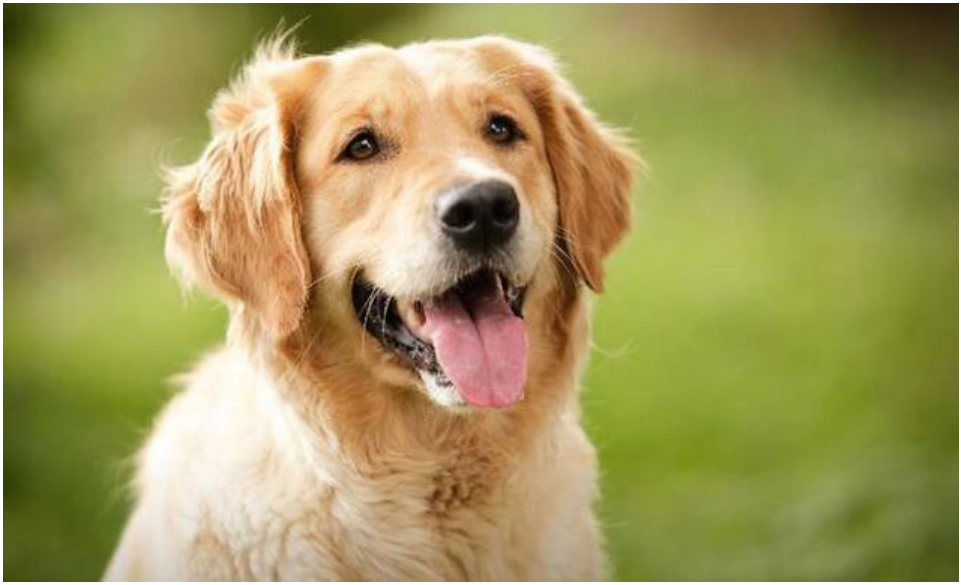
\includegraphics[width=\linewidth,height=0.5\textheight,keepaspectratio]{assets/New-Lecture-Inference_Optimisation/harvard_L11_compression_p14.png}\\[-0.4em]
  \end{columns}
  \vspace{0.4em}
\end{frame}


\begin{frame}{Distillation: Soft Targets}
  \textbf{\textcolor{blue}{While training, our confidence in the labels must be high.}}\\[0.8em]
  Otherwise the data would not be present in the training set.\\[1em]
  \begin{columns}[T,onlytextwidth]
    \column{0.49\textwidth}
      \small
      For example: \\[0.7em]
      \texttt{This is also a Dog}
      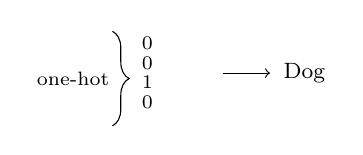
\begin{tikzpicture}[baseline={(0,0)}]
        % Draw brace + label for one-hot
        \draw[decorate,decoration={brace,amplitude=6pt,mirror}] (0,-0.2) -- (0,1) node[midway,xshift=-0.5cm] {\scriptsize one-hot};
        % One-hot vector
        \node[anchor=west] at (0.25,0.85) {\scriptsize 0};
        \node[anchor=west] at (0.25,0.60) {\scriptsize 0};
        \node[anchor=west] at (0.25,0.35) {\scriptsize 1};
        \node[anchor=west] at (0.25,0.10) {\scriptsize 0};
        % Arrow to "Dog"
        \draw[->] (1.4,0.47) -- (2,0.47);
        \node[anchor=west] at (2.05,0.47) {\footnotesize Dog};
      \end{tikzpicture}
    \column{0.48\textwidth}
      \centering
      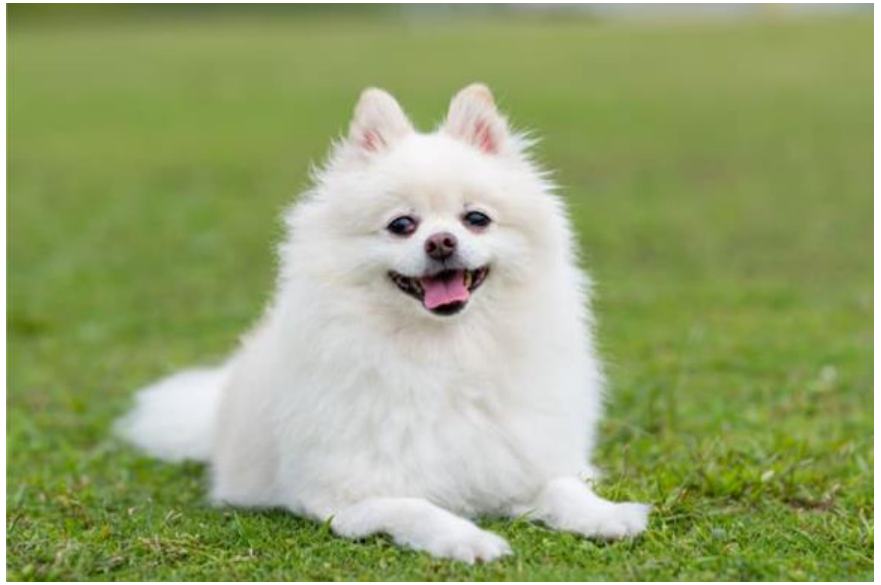
\includegraphics[width=\linewidth,height=0.5\textheight,keepaspectratio]{assets/New-Lecture-Inference_Optimisation/harvard_L11_compression_p15.png}\\[-0.4em]
  \end{columns}
  \vspace{0.4em}
\end{frame}

\begin{frame}{Distillation: Soft Targets}
  \textbf{\textcolor{blue}{While training, our confidence in the labels must be high.}}\\[0.8em]
  Otherwise the data would not be present in the training set.\\[1em]
  \begin{columns}[T,onlytextwidth]
    \column{0.49\textwidth}
      \small
      For example: \\[0.7em]
      \texttt{This is a Cat}
      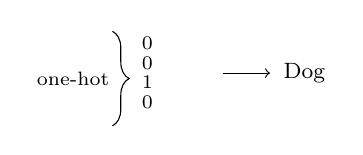
\begin{tikzpicture}[baseline={(0,0)}]
        % Draw brace + label for one-hot
        \draw[decorate,decoration={brace,amplitude=6pt,mirror}] (0,-0.2) -- (0,1) node[midway,xshift=-0.5cm] {\scriptsize one-hot};
        % One-hot vector
        \node[anchor=west] at (0.25,0.85) {\scriptsize 0};
        \node[anchor=west] at (0.25,0.60) {\scriptsize 0};
        \node[anchor=west] at (0.25,0.35) {\scriptsize 1};
        \node[anchor=west] at (0.25,0.10) {\scriptsize 0};
        % Arrow to "Dog"
        \draw[->] (1.4,0.47) -- (2,0.47);
        \node[anchor=west] at (2.05,0.47) {\footnotesize Dog};
      \end{tikzpicture}
    \column{0.48\textwidth}
      \centering
      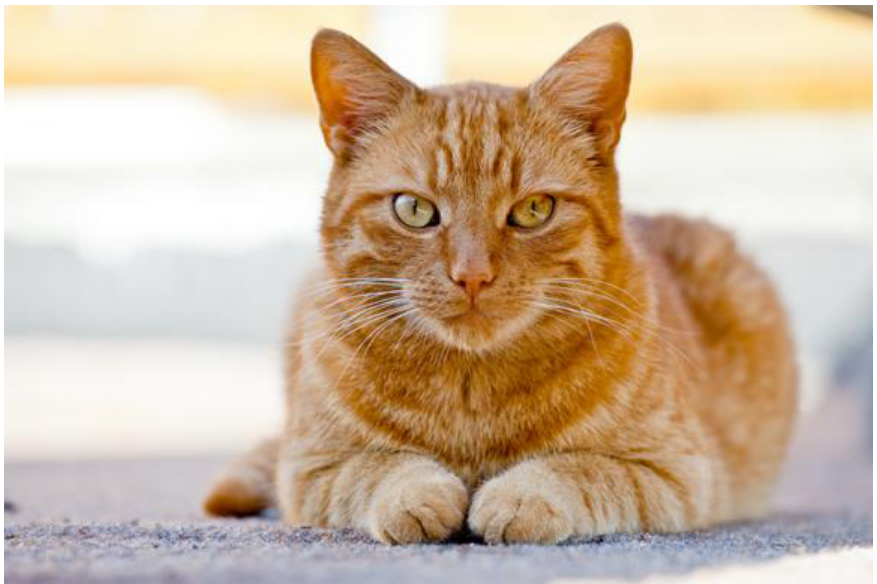
\includegraphics[width=\linewidth,height=0.5\textheight,keepaspectratio]{assets/New-Lecture-Inference_Optimisation/harvard_L11_compression_p17.png}\\[-0.4em]
  \end{columns}
  \vspace{0.4em}
\end{frame}

\begin{frame}{Distillation: Soft targets}
  \begin{columns}[T,onlytextwidth]
    \column{0.55\textwidth}
      \vspace{0.5em}
      \textbf{What about this example?}\\[1.2em]
      % Table faithfully matching slide image: 3 classes + row labels + col labels
      \setlength{\tabcolsep}{0.45em}
      \renewcommand{\arraystretch}{1.22}
      \texttt{This is a \ldots}
      \[
        \begin{pmatrix}
          0 \\
          0.5 \\
          0.5 \\
          0 \\
        \end{pmatrix}
      \]
 
    \column{0.44\textwidth}
      \centering
      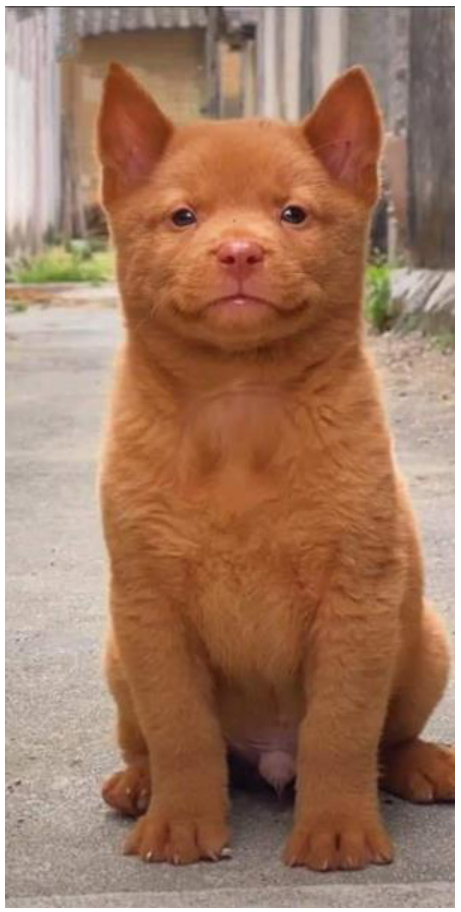
\includegraphics[width=0.78\linewidth,height=0.5\textheight,keepaspectratio]{assets/New-Lecture-Inference_Optimisation/harvard_L11_compression_p19.png}\\[0.2em]
  \end{columns}
  \vspace{0.3em}
\end{frame}

\begin{frame}{Distillation: Soft targets}
  \begin{columns}[T,onlytextwidth]
    \column{0.55\textwidth}
      \vspace{0.5em}
      In the real world, the distinction is never that clear.

      Ideally, the \href{https://en.wikipedia.org/wiki/Soft_target}{training labels must be soft}, to learn about the nuanced relations across the elements of the dataset.
 
    \column{0.44\textwidth}
      \centering
      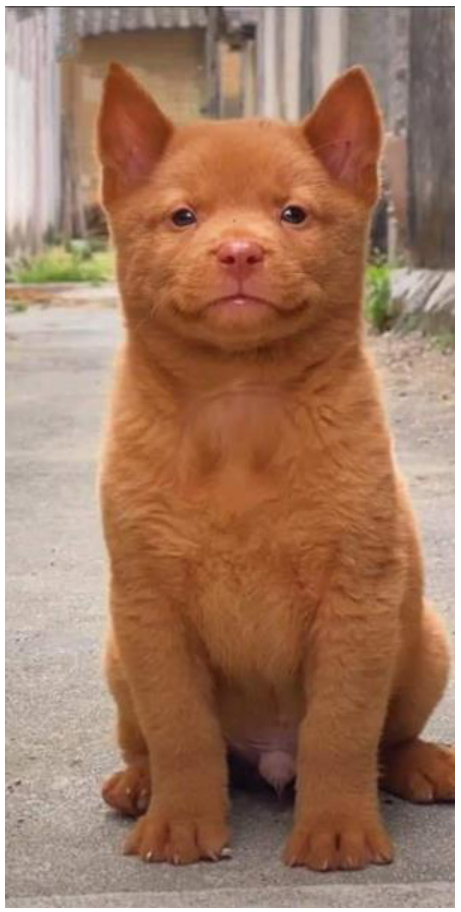
\includegraphics[width=0.78\linewidth,height=0.5\textheight,keepaspectratio]{assets/New-Lecture-Inference_Optimisation/harvard_L11_compression_p19.png}\\[0.2em]
  \end{columns}
  \vspace{0.3em}
\end{frame}

\begin{frame}{Distillation: Teacher -- Student}
  \begin{columns}[T,onlytextwidth]
    \column{0.52\textwidth}
      The teacher shows the student the \textcolor{blue}{relations} between the different classes, based on what it \textcolor{blue}{learned} during its training stage.

      \vspace{0.6em}
      From a dataset containing the original categories, the teaching outputs the \textcolor{blue}{normalized probabilities} for each example.

    \column{0.46\textwidth}
      \centering
      % Table displaying labels and probabilities, faithfully matching slide image
      \setlength{\tabcolsep}{0.45em}
      \renewcommand{\arraystretch}{1.22}
      \begin{tabular}{c|cccc}
        & \footnotesize cow & \footnotesize car & \footnotesize dog & \footnotesize cat \\
        \hline
        \footnotesize Original labels & $0$ & $1$ & $0$ & $0$ \\
        \footnotesize Probabilities & $10^{-6}$ & $0.9$ & $0.1$ & $10^{-9}$ \\
      \end{tabular}
 
      \vspace{0.6em}

      {\scriptsize
        Adapted from:\par
        Geoffrey Hinton, Oriol Vinyals \& Jeff Dean, \href{https://arxiv.org/abs/1503.02531}{\textit{Distilling the Knowledge in a Neural Network}}
      }
  \end{columns}
\end{frame}

\begin{frame}{Distillation: Teacher -- Student (Softening with Temperature)}
  \begin{columns}[T,onlytextwidth]
    \column{0.52\textwidth}
      To enhance the student's learning, the teacher \textcolor{blue}{softens} its output $z$ even more.

      \vspace{0.7em}
      To do this, introduces the softmax function with temperature $T$:

      \begin{align*}
        q_i = \frac{\exp\left(z_i / T\right)}{\sum\limits_j \exp\left(z_j / T\right)}
      \end{align*}

      \vspace{0.7em}
      \textit{“Soft” targets allow the student to learn the teacher's implicit knowledge about class similarities.}

    \column{0.46\textwidth}
      \centering
      % Table matching values from image, with original, softmax, and softened probabilities
      \setlength{\tabcolsep}{0.4em}
      \renewcommand{\arraystretch}{1.1}
      \begin{tabular}{c|cccc}
        & \footnotesize cow & \footnotesize car & \footnotesize dog & \footnotesize cat \\
        \hline
        \footnotesize Original labels & $0$ & $1$ & $0$ & $0$ \\
        \footnotesize Softmax probabilities & $10^{-6}$ & $0.9$ & $0.1$ & $10^{-9}$ \\
        \footnotesize Softened probabilities & $0.05$ & $0.3$ & $0.2$ & $0.005$
      \end{tabular}

      \vspace{0.75em}
      {\footnotesize
        Adapted from:\par
        Geoffrey Hinton, Oriol Vinyals \& Jeff Dean, \href{https://arxiv.org/abs/1503.02531}{\textit{Distilling the Knowledge in a Neural Network}}
      }
  \end{columns}
\end{frame}

\begin{frame}{Distillation: Teacher -- Student (Softening with Temperature)}
  \begin{columns}[T,onlytextwidth]
    \column{0.52\textwidth}
      A high value of $T$ will dilute the information contained in the probabilities.
      \begin{itemize}
        \item The standard softmax is recovered for $T{=}1$.
        \item For $T{>}1$, the probabilities are softened. Typical values range between $2$ and $5$.
        \item For $T{<}1$, it approaches to the original one-hot labels.
      \end{itemize}
 

    \column{0.46\textwidth}
      \centering
      % Table matching values from image, with original, softmax, and softened probabilities
      \setlength{\tabcolsep}{0.4em}
      \renewcommand{\arraystretch}{1.1}
      \begin{tabular}{c|cccc}
        & \footnotesize cow & \footnotesize car & \footnotesize dog & \footnotesize cat \\
        \hline
        \footnotesize Original labels & $0$ & $1$ & $0$ & $0$ \\
        \footnotesize Softmax probabilities & $10^{-6}$ & $0.9$ & $0.1$ & $10^{-9}$ \\
        \footnotesize Softened probabilities & $0.05$ & $0.3$ & $0.2$ & $0.005$
      \end{tabular}

      \vspace{0.75em}
      {\footnotesize
        Adapted from:\par
        Geoffrey Hinton, Oriol Vinyals \& Jeff Dean, \href{https://arxiv.org/abs/1503.02531}{\textit{Distilling the Knowledge in a Neural Network}}
      }
  \end{columns}
\end{frame}

\begin{frame}{Distillation: Teacher--Student Training}
  \begin{columns}[T,onlytextwidth]
    \column{0.47\textwidth}
      \vspace{0.5em}
      \begin{itemize}\itemsep0.7em
        \item The student is trained to both:
        \begin{itemize}
          \item Solve the original task (matching the hard/true labels).
          \item Replicate the softened probabilities (soft labels) from the teacher.
        \end{itemize}
        \item This allows the student to learn not only the correct answer, but also the teacher's representation of class similarities.
      \end{itemize}
    \column{0.53\textwidth}
      % Placeholder for image: Teacher-Student Distillation diagram
      \centering
      \fbox{
        \parbox[c][4.2cm][c]{0.92\linewidth}{
          \centering
          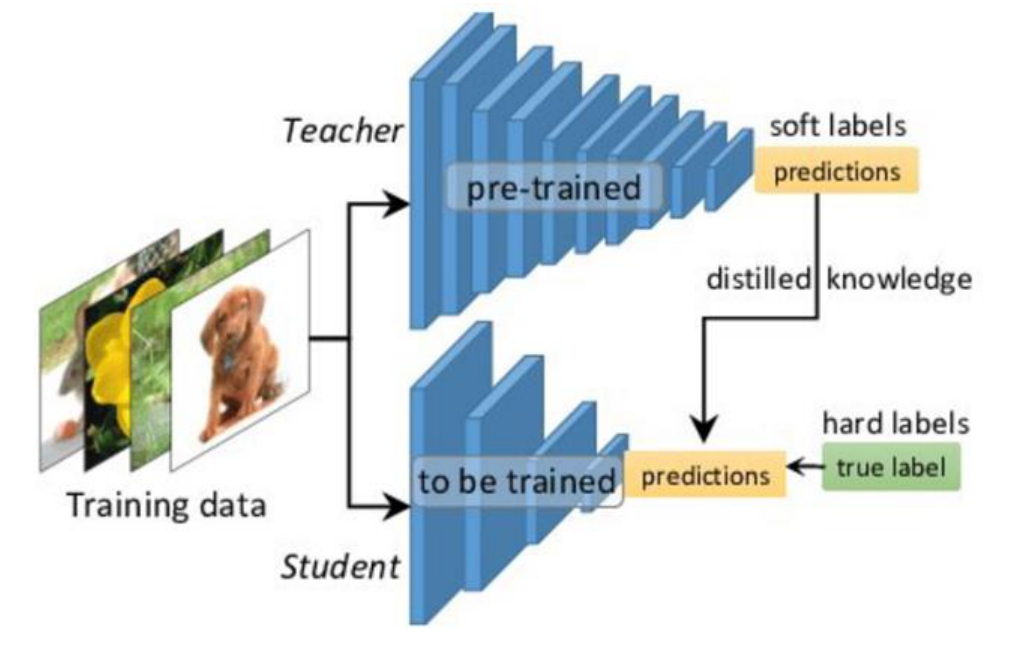
\includegraphics[width=0.78\linewidth,height=0.5\textheight,keepaspectratio]{assets/New-Lecture-Inference_Optimisation/harvard_L11_compression_p25.png}\\[0.2em]
          {\scriptsize Geoffrey Hinton, Oriol Vinyals \& Jeff Dean, \textit{Distilling the Knowledge in a Neural Network}}
     
        }
      }
      \vspace{0.5em}

      % If desired, can also include something like:
      % \includegraphics[width=\linewidth,keepaspectratio]{assets/New-Lecture-Inference_Optimisation/teacher_student_distillation.png}\\
      % {\scriptsize Geoffrey Hinton, Oriol Vinyals \& Jeff Dean, \textit{Distilling the Knowledge in a Neural Network}}
  \end{columns}
\end{frame}

\begin{frame}{Distillation: Teacher--Student Scenarios}
  \vspace{0.6em}
  \textbf{Scenario 1:}
  \begin{itemize}
    \item[] Train on the same data as the teacher model. \\
      {\scriptsize (DistilBERT was trained on this example.)}
  \end{itemize}
  \vspace{0.5em}
  \textbf{Scenario 2:}
  \begin{itemize}
    \item[] Train on a reduced dataset. This is usually done when you have the teacher model but not the original dataset or resources.
  \end{itemize}
  \vspace{1em}
  % Optionally, add a horizontal line or adjust spacing for clarity
\end{frame}

\begin{frame}{Distillation: Teacher--Student Loss}
  \begin{columns}[T,onlytextwidth]
    \column{0.54\textwidth}
      It minimizes the sum of two different cross-entropy functions:
      \begin{itemize}
        \item One involving the original hard labels obtained using a softmax with $T = 1$.
        \item One involving the softened probabilities with $T > 1$.
      \end{itemize}
    \column{0.42\textwidth}
      \centering
      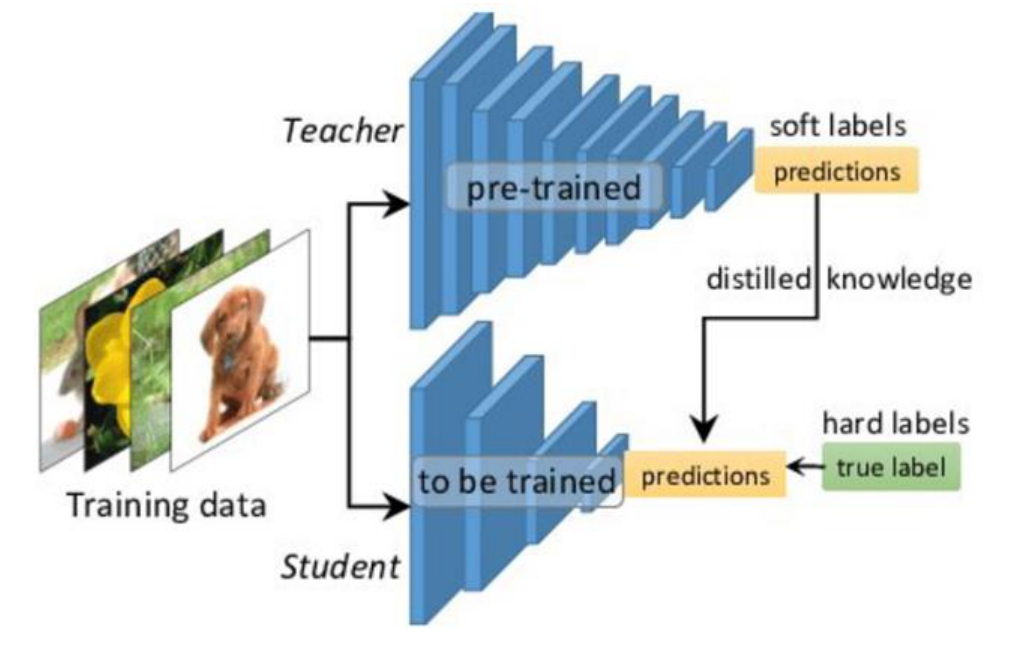
\includegraphics[width=0.98\linewidth,height=0.5\textheight,keepaspectratio]{assets/New-Lecture-Inference_Optimisation/harvard_L11_compression_p25.png}\\[0.2em]
      {\scriptsize Geoffrey Hinton, Oriol Vinyals \& Jeff Dean, \textit{Distilling the Knowledge in a Neural Network}}
  \end{columns}
\end{frame}

\begin{frame}{Distillation: Teacher--Student}
  \centering
  % Use the referenced slide as a visual explanation for training process
  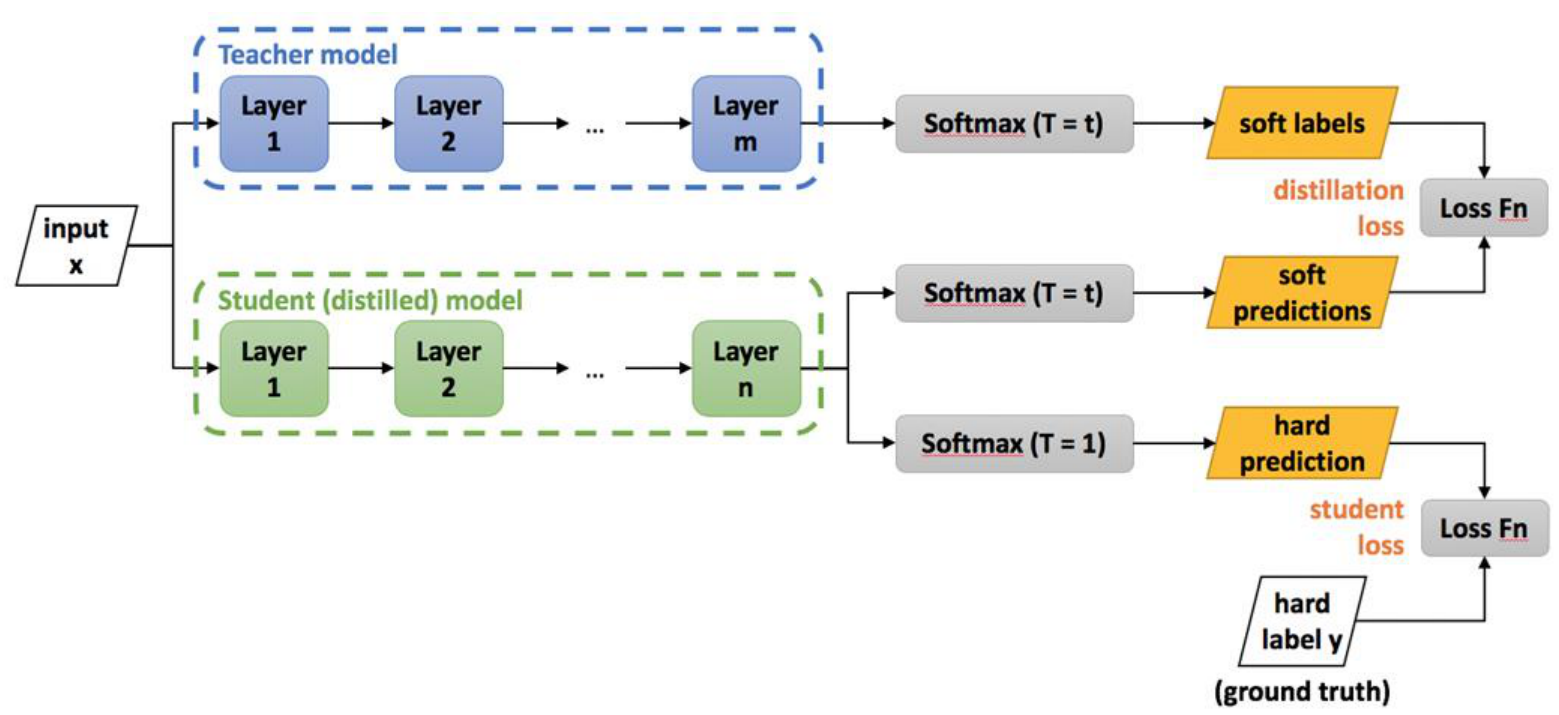
\includegraphics[width=0.97\linewidth,height=0.8\textheight,keepaspectratio]{assets/New-Lecture-Inference_Optimisation/harvard_L11_compression_p28.png}\\[0.4em]
  {\scriptsize Reference: Geoffrey Hinton, Oriol Vinyals \& Jeff Dean, \textit{Distilling the Knowledge in a Neural Network}.}
  \vspace{1em}
  
  \[
    L = \lambda L_{\mathrm{student}} + (1-\lambda) L_{\mathrm{distillation}}
  \]
\end{frame}

\begin{frame}{Distillation: Teacher--Student Training}
  \centering
  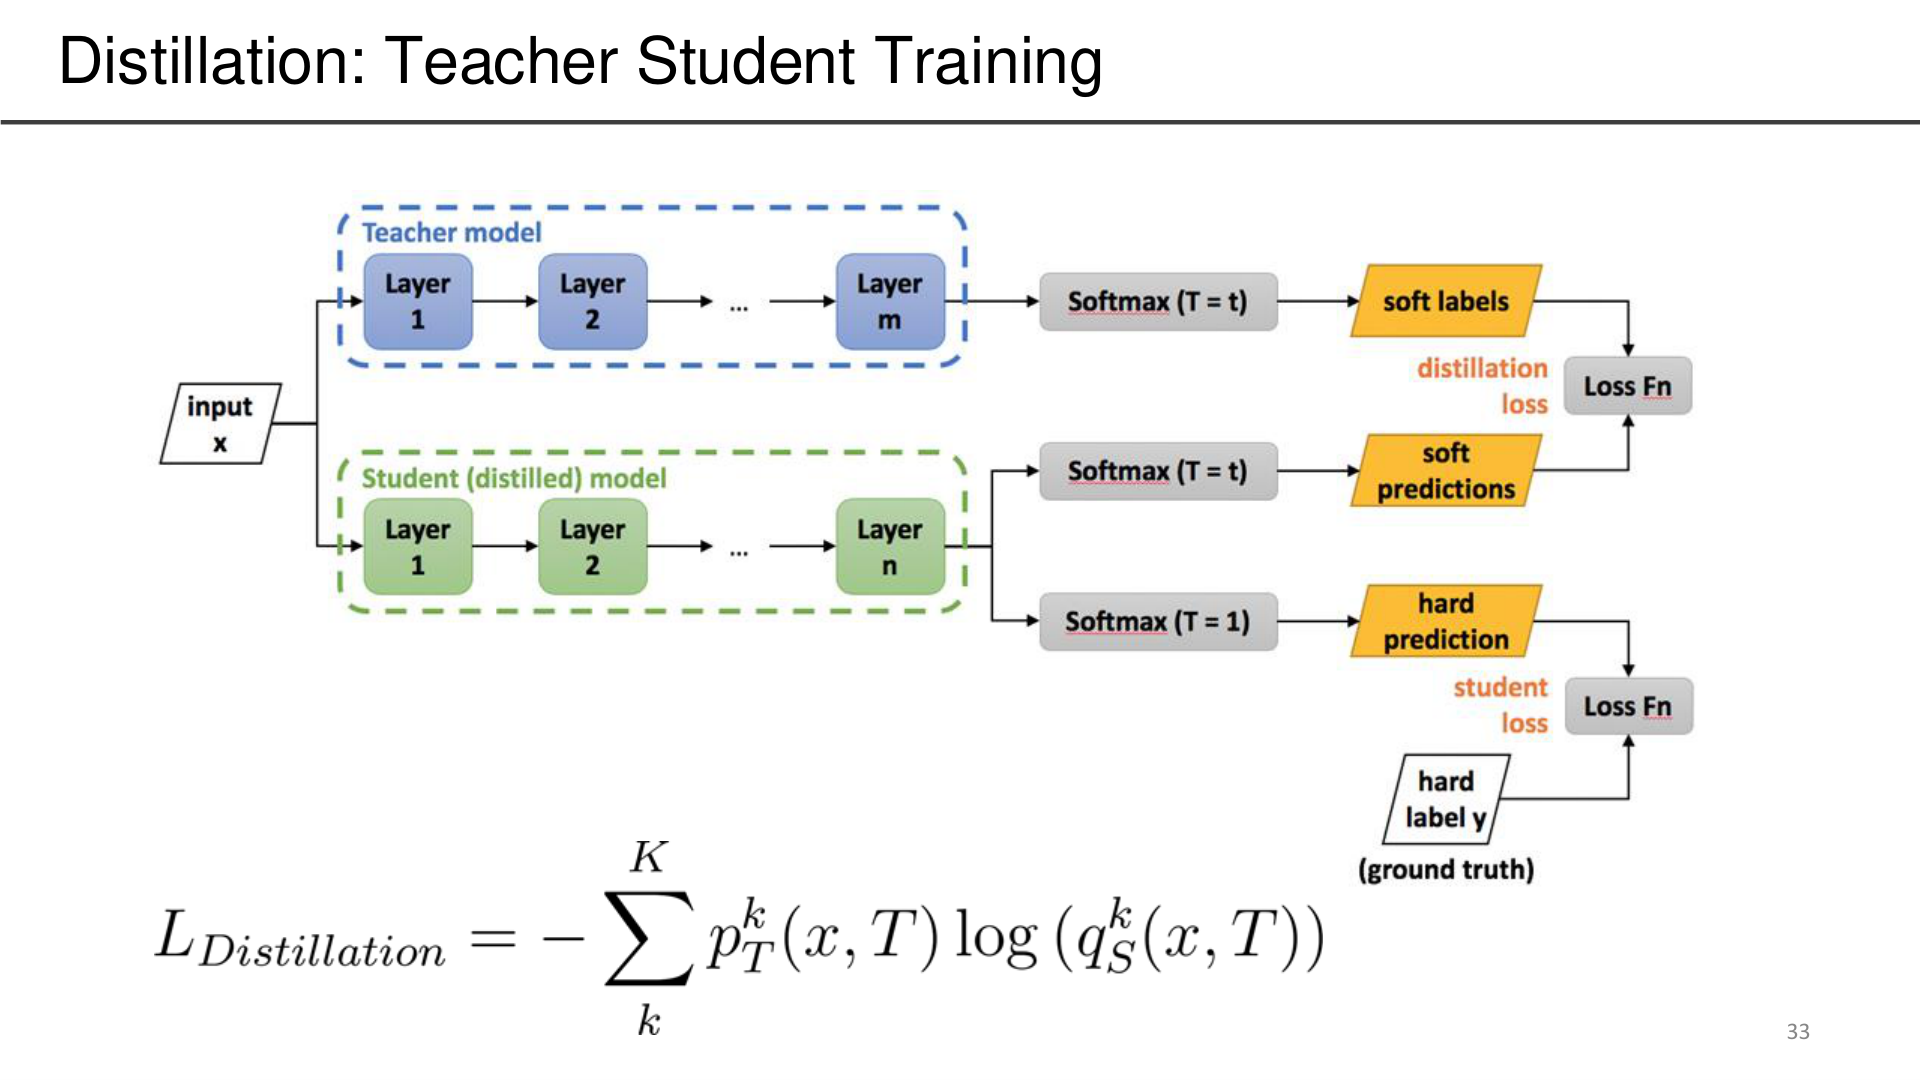
\includegraphics[width=0.97\linewidth,height=0.8\textheight,keepaspectratio]{assets/New-Lecture-Inference_Optimisation/harvard_L11_compression_p29.png}\\[0.4em]
\end{frame}

\begin{frame}{Distillation: Teacher--Student}
  \small
  \[
    L_\mathrm{Distillation} = -\sum_{k=1}^{K} p_T^k(x, T)\log\big(q_S^k(x, T)\big)
  \]
  \vspace{0.8em}

  In our example, for the example $n$ in the dataset:
  \[
    p_T(x, T) = [0.05,\ 0.3,\ 0.2,\ 0.005]
  \]

  And our predictions
  \[
    q_T(x, T) = [0.1,\ 0.45,\ 0.30,\ 0.15]
  \]

  The resulting loss value for this example is:
  \[
    -\Big[0.05 \cdot \log(0.1)\ +\ 0.3 \cdot \log(0.45)\ +\ 0.2 \cdot \log(0.30)\ +\ 0.005 \cdot \log(0.15)\Big]
  \]
\end{frame}
